PINN losses involve differential operators of the neural network, for instance the Laplacian.
Recently, \citet{li2023forward} proposed a new computational framework called \emph{forward Laplacian} to evaluate the Laplacian and the neural network's prediction in one forward traversal.
To establish a Kronecker-factorized approximation of the Gramian, which consists of the Laplacian's gradient, we need to know how a weight matrix enters its computation.
Here, we describe how the weight matrix of a linear layer inside a feed-forward net enters the Laplacian's computation when using the forward Laplacian framework.
We start by connecting the forward Laplacian framework to Taylor-mode automatic differentiation \citep{griewank2008evaluating,bettencourt2019taylor}, both to make the presentation self-contained and to explicitly point out this connection which we believe has not been done previously.

\subsection{Taylor-Mode Automatic Differentiation}\label{sec:taylor-mode-tutorial}
The idea of Taylor-mode is to forward-propagate Taylor coefficients, i.e.\,directional derivatives, through the computation graph. We provide a brief summary based on its description in \cite{bettencourt2019taylor}.

\paragraph{Taylor series and directional derivatives} Consider a function $f: \sR^d \to \sR$ and its $K$-th order Taylor expansion at a point $\vx \in \sR^d$ along a direction $\alpha \vv \in \sR^d$ with $\alpha \in \sR$,
\begin{align*}
  \hat{f}(\alpha) =
  f(\vx + \alpha \vv)
  &=
    f(\vx)
    +
    \alpha
    \left(
    \frac{\partial f(\vx)}{\partial \vx}
    \right)^{\top} \vv
    +
    \frac{\alpha^2}{2!}
    \vv^\top
    \left(
    \frac{\partial^2 f(\vx)}{\partial \vx^2}
    \right) \vv
  \\
  &\phantom{=}+
    \frac{\alpha^3}{3!}
    \sum_{i_1, i_2 i_3}
    \left(
    \frac{\partial^3 f(\vx)}{\partial\vx^3}
    \right)_{i_1, i_2, i_3} \evv_{i_1} \evv_{i_2} \evv_{i_3}
  \\
  &\phantom{=}+
    \ldots
  \\
  &\phantom{=}+
    \frac{\alpha^K}{K!}
    \sum_{i_1, \dots, i_K}
    \left(
    \frac{\partial^K f(\vx)}{\partial\vx^K}
    \right)_{i_1, \dots, i_K} \evv_{i_1} \cdots \evv_{i_K}\,.
\end{align*}
We can unify this expression by introducing the $K$-th order directional derivative of $f$ at $\vx$ along $\vv$,
\begin{align*}
  \partial^K f(\vx)
  \underbrace{\left[ \vv, \ldots, \vv \right]}_{K\,\text{times}}
  \coloneqq
  \sum_{i_1, \dots, i_K}
  \left(
  \frac{\partial^K f(\vx)}{\partial\vx^K}
  \right)_{i_1, \dots, i_K} \evv_{i_1} \dots \evv_{i_K}\,.
\end{align*}
This simplifies the uni-directional Taylor expansion to
\begin{align*}
  \hat{f}(\alpha) = f(\vx + \alpha\vv)
  &=
    f(\vx)
    +
    \alpha
    \partial f(\vx)[\vv]
    +
    \frac{\alpha^2}{2!}
    \partial^2 f(\vx)[\vv, \vv]
    +
    \frac{\alpha^3}{3!}
    \partial^3 f(\vx)[\vv, \vv, \vv]
  \\
  &\phantom{=}+
    \ldots
    +
    \frac{\alpha^K}{K!}
    \partial^K f(\vx)[\vv, \ldots, \vv]
  \\
  &\eqqcolon
    \sum_{k=1}^K
    \frac{\alpha^k}{k!}
    \partial^k f(\vx)\left[\otimes^k \vv  \right]
    \eqqcolon
    \sum_{k=1}^K
    w^f_k \alpha^k
\end{align*}
where we have used the notation $\otimes^k \vv$ to indicate $k$ copies of $\vv$, and introduced the $k$-th order Taylor coefficient $w^f_k \in \sR$ of $f$.
This generalizes to vector-valued functions:
If $f$'s output was vector-valued, say $f(\vx) \in \sR^c$, we would have Taylor-expanded each component individually and grouped coefficients of same order into vectors $\vw_k^f \in \sR^c$ such that $[\vw_k^f]_i$ is the $k$-th order Taylor coefficient of the $i$th component of $f$.

\paragraph{A note on generality:} In this introduction to Taylor-mode, we limit the discussion to the computation of higher-order derivatives along a single direction $\vv$, i.e.\,$\partial^Kf(\vx)[\vv, \dots, \vv]$.
This is limited though, e.g.\,if we set $K=2$ then we can compute $\partial^2 f(\vx)[\vv, \vv] = \vv^{\top} (\nicefrac{\partial^2 f(\vx)}{\partial\vx^2}) \vv$.
We can set $\vv = \ve_i$ to the $i$-th standard basis vector to compute the $i$-th diagonal element of the Hessian.
But we cannot evaluate off-diagonal elements, as this would require multi-directional derivatives, like $\partial^2 f(\vx) [\ve_i, \ve_{j\neq i}]$.
A more general description of Taylor-mode for multi-directional Taylor series along $M$ directions, $\hat{f}(\alpha_1, \dots, \alpha_M) = f(\vx + \alpha_1 \vv_1 + \dots + \alpha_M \vv_M)$, which require more general directional derivatives $\partial^K f(\vx) [\vv_1, \dots, \vv_K]$ (each vector can be different) are discussed in \cite{johnson2021taylor-made}.
We will use this formulation later to generalize the forward Laplacian scheme to more general weighted sums of second-order derivatives in \Cref{sec:generalized-forward-laplacian}.

\paragraph{Composition rule}
Next, we consider the case where $f = g \circ h$ is a composition of two functions. Starting from the Taylor coefficients $\vw_0^h, \dots \vw_K^h$ of $\hat{h}(\alpha) = h(\vx + \alpha \vv)$, the Taylor coefficients $\vw_0^f, \dots, \vw_K^f$ of $\hat{f}(\alpha) = f(\vx + \alpha\vv)$ follow from Fa\`a di Bruno's formula~\cite{griewank2008evaluating,bettencourt2019taylor}:
\begin{align}\label{eq:taylor-mode-forward}
  \vw_{k}^f
  =
  \sum_{\sigma \in \mathrm{part}(k)}
  \frac{1}{n_1! \dots n_K!}
  \partial^{|\sigma|}g(\vw_0^h)
  \left[
  \otimes_{s \in \sigma}
  \vw_s^h
  \right]
\end{align}
In the above, $\mathrm{part}(k)$ is the set of all integer partitionings of $k$; a set of sets. $|\sigma|$ denotes the length of a set $\sigma \in \mathrm{part}(k)$, $n_i$ is the count of integer $i$ in $\sigma$, and $\vw_0^h = h(\vx)$.

\textbf{Second-order Taylor-mode} Our goal is the computation of second-order derivatives of $f$ w.r.t.\,$\vx$.
So let's work out \Cref{eq:taylor-mode-forward} up to order $K=2$.
The zeroth and first order are simply the forward pass and the forward-mode gradient chain rule.
For the second-order term, we need the integer partitioning of 2, given by $\mathrm{part}(2) = \left\{ \{1, 1\}, \{2\} \right\}$.
This results in
\begin{subequations}\label{eq:taylor-mode-second-order}
  \begin{align}
    \vw_0^f
    &=
      g(\vw_0^h)\,,
    \\
    \vw_1^f
    &=
      \partial g(\vw_0^h)[\vw_1^h]\,,
    \\
    \vw_2^f
    &=
      \frac{1}{2}
      \partial^2 g(\vw_0^h)[\vw_1^h, \vw_1^h]
      +
      \partial g(\vw_0^h)[\vw_2^h]\,.
  \end{align}
\end{subequations}
We can also express $\vw_1^f, \vw_2^f$ in terms of Jacobian- and Hessian-vector products of $g$,
\begin{subequations}\label{eq:taylor-mode-second-order-jac-hess}
  \begin{align}
    \label{eq:taylor-mode-second-order-jac}
    \vw_1^f
    &=
      \left(
      \jac_{\vw_0^h} g(\vw_0^h)
      \right) \vw_1^h\,,
    \\
    \vw_2^f
    &=
      \frac{1}{2}
      \begin{pmatrix}
        {\vw_1^h}^{\top}
        \frac{
        \partial^2 \left[ g(\vw_0^h) \right]_1
        }{
        \partial{\vw_0^h}^2
        }
        \vw_1^h
        \\
        \vdots
        \\
        {\vw_1^h}^{\top}
        \frac{
        \partial^2 \left[ g(\vw_0^h) \right]_D
        }{
        \partial{\vw_0^h}^2
        }
        \vw_1^h
      \end{pmatrix}
      +
      \left(
      \jac_{\vw_0^h} g(\vw_0^h)
      \right) \vw_2^h\,.
  \end{align}
\end{subequations}
Note that first-order Taylor-mode (\Cref{eq:taylor-mode-second-order-jac}) corresponds to the standard forward-mode autodiff which pushes forward error signals through Jacobian-vector products.

\subsection{Forward Laplacian}
Our goal is to compute the Laplacian of $f: \sR^d \to \sR^c$ (in practise, $c=1$),
\begin{align}
  \Delta_{\vx} f(\vx)
  =
  \sum_{i=1}^d
  \begin{pmatrix}
    \partial^2[f(\vx)]_1[\ve_i, \ve_i]
    \\
    \vdots
    \\
    \partial^2[f(\vx)]_c[\ve_i, \ve_i]
  \end{pmatrix}
  \coloneq
  2 \sum_{i=1}^d \vw_{2,i}^f \in \sR^c\,,
\end{align}
where $\ve_i$ is the $i$-th standard basis vector, $[f(\vx)]_j$ is the $j$-th component of $f(\vx)$, and we have introduced the second-order Taylor coefficients $\vw_{2,i}^f$ of $f$ along $\ve_i$.
The Laplacian requires computing, then summing, the second-order Taylor coefficients of $d$ Taylor approximations $\{f(\vx + \ve_i)\}_{i=1,\dots, d}$.

\paragraph{Naive approach} We can use Taylor-mode differentiation to compute all these components in one forward traversal. Adding the extra loop over the Taylor expansions we want to compute in parallel, we obtain the following scheme from \Cref{eq:taylor-mode-second-order},
\begin{subequations}\label{eq:taylor-mode-naive-laplacian}
  \begin{align}
    \vw_0^f
    &=
      g(\vw_0^h)\,,
    \\
    \left\{
    \vw_{1,i}^f
    \right\}_{i=1, \dots, d}
    &=
      \left\{
      \partial g(\vw_0^h)[\vw_{1,i}^h]
      \right\}_{i=1, \dots, d}\,,
    \\ \label{eq:naive-laplacian-second-order-term}
    \left\{
    \vw_{2,i}^f
    \right\}_{i=1, \dots, d}
    &=
      \left\{
      \frac{1}{2}
      \partial^2 g(\vw_0^h)[\vw_{1,i}^h, \vw_{1,i}^h]
      +
      \partial g(\vw_0^h)[\vw_{2,i}^h]
      \right\}_{i=1, \dots, d}\,.
  \end{align}
\end{subequations}

\paragraph{Forward Laplacian framework}
Computing the Laplacian via \Cref{eq:taylor-mode-naive-laplacian} first computes, then sums, the diagonal second-order derivatives $\{ \vw_{2,i}^f \}_{i=1,\dots, d}$.
Note that we can pull the sum inside the forward propagation scheme, specifically \Cref{eq:naive-laplacian-second-order-term}, and push-forward the summed second-order coefficients. This simplifies \Cref{eq:taylor-mode-naive-laplacian} to
\begin{subequations}\label{eq:forward-laplacian}
  \begin{align}
    \vw_0^f
    &=
      g(\vw_0^h)\,,
    \\
    \left\{
    \vw_{1,i}^f
    \right\}_{i=1, \dots, d}
    &=
      \left\{
      \partial g(\vw_0^h)[\vw_{1,i}^h]
      \right\}_{i=1, \dots, d}\,,
    \\
    \underbrace{
    \sum_{i=1}^d
    \vw_{2,i}^f
    }_{\nicefrac{1}{2}\Delta_{\vx} f(\vx)}
    &=
      \left(
      \frac{1}{2}
      \sum_{i=1}^d
      \partial^2 g(\vw_0^h)[\vw_{1,i}^h, \vw_{1,i}^h]
      \right)
      +
      \partial g(\vw_0^h)
      \underbrace{
      \left[
      \sum_{i=1}^d \vw_{2,i}^h
      \right]
      }_{\nicefrac{1}{2}\Delta_{\vx} g(\vx)}\,.
  \end{align}
\end{subequations}
\Cref{eq:forward-laplacian} is the forward Laplacian framework from \citet{li2023forward} for computing the Laplacian of a neural network.
Here, we have derived it from Taylor-mode automatic differentiation.
Note that \Cref{eq:forward-laplacian} requires less computations and memory than \Cref{eq:taylor-mode-naive-laplacian} because we can pull the summation from the Laplacian into the forward propagation scheme.

\subsubsection{Forward Laplacian for Elementwise Activation Layers}
We now describe \Cref{eq:forward-laplacian} for the case where $g: \sR^c \to \sR^c$ acts element-wise via $\sigma: \sR \to \sR$.
We will write $\sigma(\bullet), \sigma'(\bullet), \sigma''(\bullet)$ to indicate element-wise application of $\sigma$, its first derivative $\sigma'$, and second derivative $\sigma''$ to all elements of $\bullet$.
Further, let $\odot$ denote element-wise multiplication, and $(\bullet)^{\odot 2}$ element-wise squaring.
With that, we can write the Jacobian as $\jac_{h(\vx)}g(\vx) = \diag(\sigma(h(\vx)))$ where $\diag(\bullet)$ embeds a vector $\bullet$ into the diagonal of a matrix.
The Hessian of component $i$ is $\nicefrac{\partial^2 [g(h(\vx))]_i}{\partial h(\vx)^2} = [\sigma''(h(\vx))]_i \ve_i \ve_i^{\top}$.
Inserting \Cref{eq:taylor-mode-second-order-jac-hess} into \Cref{eq:forward-laplacian} and using the Jacobian and Hessian expressions of the element-wise activation function yields the following forward Laplacian forward propagation:
\begin{subequations}\label{eq:forward-laplacian-activation-layers}
  \begin{align}
    \vw_0^f
    &=
      \sigma(\vw_0^h)\,,
    \\
    \left\{ \vw_{1,i}^f \right\}
    &=
      \left\{ \sigma'(\vw_0^h) \odot \vw_{1,i}^h \right\}_{i=1, \dots, d}\,,
    \\
    \sum_{i=1}^d \vw_{2,i}^f
    &=
      \frac{1}{2}
      \sigma''(\vw_0^h) \odot
      \left(
      \sum_{i=1}^d
      \left(\vw_{1,i}^h\right)^{\odot 2}
      \right)
      +
      \sigma'(\vw_0^h)
      \odot
      \left(
      \sum_{i=1}^d \vw_{2,i}^h
      \right)\,.
  \end{align}
\end{subequations}

\subsubsection{Forward Laplacian for Linear Layers}
Now, let $g: \sR^{D_{\text{in}}} \to \sR^{D_{\text{out}}}$ be a linear layer with weight matrix $\mW \in \sR^{D_{\text{out}} \times D_{\text{in}}}$ and bias vector $\vb \in \sR^{D_{\text{out}}}$.
Its Jacobian is $\jac_{h(\vx)}( \mW h(\vx) + \vb) = \mW$ and the second-order derivative is zero.
Hence, \Cref{eq:forward-laplacian} for linear layers becomes
\begin{subequations}\label{eq:forward-laplacian-linear-layer}
  \begin{align}
    \vw_0^f
    &=
      \mW \vw_0^h + \vb\,,
    \\
    \left\{ \vw_{1,i}^f \right\}_{i=1, \dots, d}
    &=
      \left\{ \mW \vw_{1,i}^h \right\}_{i=1, \dots, d}\,,
    \\
    \sum_{i=1}^d \vw_{2,i}^f
    &=
      \mW
      \left( \sum_{i=1}^d \vw_{2,i}^h\right)\,.
  \end{align}
\end{subequations}
We can summarize \Cref{eq:forward-laplacian-linear-layer} in a single equation by grouping all quantities that are multiplied by $\mW$ into a single matrix, and appending a single row of ones or zeros to account for the bias:
\begin{align}
  \nonumber
  \underbrace{
  \begin{pmatrix}
    \vw_0^f
    &
      \vw_{1,1}^f
    &
      \dots
    &
      \vw_{1,d}^f
    &
      \sum_{i=1}^D \vw_{2,i}^f
  \end{pmatrix}
  }_{\coloneq \mT^f \in \sR^{D_{\text{out}} \times (d+2)}}
  &=
    \begin{pmatrix}
      \mW & \vb
    \end{pmatrix}
    \underbrace{
    \begin{pmatrix}
      \vw_0^h
      &
        \vw_{1,1}^h
      &
        \dots
      &
        \vw_{1,d}^h
      &
        \sum_{i=1}^d \vw_{2,i}^h
      \\
      1 & 0 & \dots & 0 & 0
    \end{pmatrix}
    }_{\coloneq \mT^h \in \sR^{(D_{\text{in}} +1) \times (d+2)}}\,,
    \shortintertext{or, in compact form,}
    \mT^f
  &=
    \tilde{\mW}
    \mT^h\,.
    \label{eq:forward-laplacian-linear-layer-compact}
\end{align}
\Cref{eq:forward-laplacian-linear-layer-compact} shows that the weight matrix $\tilde{\mW}^{(l)} = (\mW^{(l)} \ \vb^{(l)})$ of a linear layer $f^{(l)}$ inside a neural network $f^{(L)} \circ \ldots \circ f^{(1)}$ is applied to a matrix $\mT^{(l-1)} \in \sR^{D_{\text{in}}\times (d+2)}$ during the computation of the net's prediction and Laplacian via the forward Laplacian framework and yields another matrix $\mT^{(l)} \in \sR^{D_{\text{out}}\times (d+2)}$.

\subsection{Generalization of the Forward Laplacian to Weighted Sums of Second Derivatives}\label{sec:generalized-forward-laplacian}
The Laplacian is of the form $\Delta_{\vx}f = \sum_{i} \partial^2f(\vx)[\ve_i, \ve_i]$ and we previously described the forward Laplacian framework of \citet{li2023forward} as a consequence of pulling the summation into Taylor-mode's forward propagation.
Here, we derive the forward propagation to more general operators of the form $\sum_{i,j} c_{i,j} \partial^2f(\vx)[\ve_i, \ve_j]$, which contain the Laplacian for $c_{i,j} = \delta_{i,j}$.

As mentioned in \Cref{sec:taylor-mode-tutorial}, this requires a generalization of Taylor-mode which computes derivatives of the form $\partial^K f(\vx) [\vv, \dots, \vv]$, where the directions $\vv$ must be identical. We start with the formulation in \cite{johnson2021taylor-made} which expresses the $K$-th multi-directional derivative of a function $f = g \circ h$ through the composites' derivatives (all functions can be vector-to-vector)
\begin{align}
  \label{eq:taylor-mode-multi-directional}
  \partial^K f(\vx)[\vv_1, \dots, \vv_K]
  & =
  \sum_{\sigma \in \mathrm{part}(\{1, \dots, K\})}
  \partial^{|\sigma|}g(h(\vx))
  \left[
  \otimes_{\eta \in \sigma} \partial^{|\eta|}h(\vx) \left[ \otimes_{l \in \eta} \vv_l \right]
  \right]
  %\\ &
  %= \sum_{\lvert\alpha\rvert = K}
  %\partial^{\alpha}g(h(\vx))
  %\vv^\alpha
  \,.
\end{align}
Here, $\mathrm{part}(\{1, \dots, K\})$ denotes the set of all set partitions of $\{1, \dots, K\}$ ($\sigma$ is a set of sets). E.g.,
\begin{align*}
  \mathrm{part}(\{1\})
  &=
    \{
    \{ \{1 \} \}
    \}\,,
  \\
  \mathrm{part}(\{1,2\})
  &=
    \{
    \{ \{1,2\} \}, \{ \{1\}, \{2\} \}
    \}\,,
  \\
  \mathrm{part}(\{1,2,3\})
  &=
    \{
    \{ \{1,2,3\} \},
    \{ \{1\}, \{2,3\} \},
    \{ \{1,2\}, \{3\} \},
    \{ \{1,3\}, \{2\} \},
    \{ \{1\}, \{2\}, \{3\} \}
    \}\,.
\end{align*}
To make this more concrete, let's consider \Cref{eq:taylor-mode-multi-directional} for first- and second-order derivatives,
\begin{subequations}\label{eq:taylor-mode-multi-directional-1-2}
  \begin{align}
    \partial f(\vx) [\vv]
    &=
      \partial g(h(\vx)) [\partial h(\vx) [\vv]]\,,
    \\  \label{subeq:taylor-mode-multi-directional-1-2}
    \partial^2 f(\vx) [\vv_1, \vv_2]
    &=
      \partial g^2(h(\vx)) [\partial h(\vx) [\vv_1], \partial h(\vx) [\vv_2]]
      +
      \partial g(h(\vx)) [\partial h^2(\vx) [\vv_1, \vv_2]]\,.
  \end{align}
\end{subequations}

From \Cref{eq:taylor-mode-multi-directional-1-2}, we can see that if we want to compute a weighted sum of second-order derivatives $\sum_{i,j} c_{i,j} \partial^2 f(\vx)[\vv_i, \vv_j]$, we can pull the sum inside the second equation,
\begin{align}\label{eq:taylor-mode-multi-directional-1-2-sum-inside}
  \begin{split}
    \sum_{i,j} c_{i,j} \partial^2 f(\vx) [\vv_i, \vv_j]
    &=
      \sum_{i,j} c_{i,j} \partial^2 g(h(\vx)) [\partial h(\vx) [\vv_i], \partial h(\vx) [\vv_j]]
    \\
    &\phantom{=}+
      \partial g(h(\vx))
      \left[
      \sum_{i,j} c_{i,j}
      \partial^2 h(\vx) [\vv_i, \vv_j]
      \right]\,.
  \end{split}
\end{align}
Hence, we can propagate the collapsed second-order derivatives, together with all first-order derivatives along $\vv_1, \vv_2, \dots$. The only difference to the forward Laplacian is how second-order effects of an operation are incorporated (first term in \Cref{eq:taylor-mode-multi-directional-1-2-sum-inside}).

We now specify~\Cref{eq:taylor-mode-multi-directional,eq:taylor-mode-multi-directional-1-2-sum-inside} for linear layers and element-wise activation functions.

For a linear layer $g: h(\vx) \mapsto \mW h(\vx) + \vb$, we have $\partial^{m>1}g(h(x))[\vv_1, \dots, \vv_m] = \vzero$, and thus
\begin{subequations}\label{eq:taylor-mode-multi-directional-1-2-linear}
  \begin{align}
    \partial f(x) [\vv]
    &=
      \mW \partial h(x) [\vv]\,,
    \\
    \partial^2 f(x) [\vv_1, \vv_2]
    &=
      \mW \partial^2 h(x) [\vv_1, \vv_2]\,,
    \\
    \partial^K f(x) [\vv_1, \dots, \vv_K]
    &=
      \mW \partial^K h(x) [\vv_1, \dots, \vv_K]\,.
  \end{align}
\end{subequations}
The last equation is because only the set partition $\{1, \dots, K\}$ contributes to \Cref{eq:taylor-mode-multi-directional}.

For elementwise activations $g: h(x) \mapsto \sigma(h(x))$ with $\sigma: \sR \to \sR$ applied component-wise, we have the structured derivative tensor $[\partial^{m}g(h(x))]_{i_1, \dots, i_m} = \partial^m\sigma(h(x)_{i_1}) \delta_{i_1, \dots, i_m}$ and multi-directional derivative $\partial^K g(h(\vx))[\vv_1, \dots, \vv_K] = \partial^K\sigma(\vx) \odot \vv_1 \odot \dots \odot \vv_K$. \Cref{eq:taylor-mode-multi-directional-1-2} becomes
\begin{subequations}\label{eq:taylor-mode-multi-directional-1-2-activation}
  \begin{align}
    \partial f(x) [\vv]
    &=
      \sigma'(h(x)) \odot \partial h(x) [\vv]\,,
    \\
    \partial^2 f(x) [\vv_1, \vv_2]
    &=
      \sigma''(h(x)) \odot \partial h(x) [\vv_1] \odot \partial h(x) [\vv_2]
      +
      \sigma'(h(x)) \odot \partial^2 h(x) [\vv_1, \vv_2]\,.
  \end{align}
\end{subequations}
As shown in \Cref{subeq:taylor-mode-multi-directional-1-2}, for both \Cref{eq:taylor-mode-multi-directional-1-2-linear,eq:taylor-mode-multi-directional-1-2-activation}, we can pull the summation inside the propagation scheme. Specifically, to compute $\sum_{i,j} c_{i,j}\partial^2f(\vx)[\ve_i, \ve_j]$, we have for linear layers
\begin{subequations}
  \begin{align}
    f(\vx)
    &=
      g(h(\vx))\,,
    \\
    \partial f(\vx) [\ve_i]
    &=
      \mW \partial h(\vx) [\ve_i]\,,
      \qquad
      i=1, \dots, d\,,
    \\
    \textcolor{maincolor}{\sum_{i,j} c_{i,j} \partial^2 f(\vx) [\ve_i, \ve_j]}
    &=
      \mW
      \left(
      \textcolor{maincolor}{\sum_{i,j} c_{i,j} \partial^2 h(\vx) [\ve_i, \ve_j]}
      \right)\,.
  \end{align}
  and for activation layers
  \begin{align}
    f(\vx)
    &=
      \sigma(h(\vx))\,,
    \\
    \partial f(\vx) [\ve_i]
    &=
      \sigma'(h(\vx)) \odot \partial h(\vx) [\ve_i]\,,
      \qquad
      i=1, \dots, d\,,
    \\
    \begin{split}
      \textcolor{maincolor}{\sum_{i,j} c_{i,j} \partial^2 f(\vx) [\ve_i, \ve_j]}
      &=
        \sum_{i,j} c_{i,j}
        \sigma''(h(\vx)) \odot \partial h(\vx) [\ve_i] \odot \partial h(\vx) [\ve_j]
      \\
      &\phantom{=}+
        \sigma'(h(\vx))
        \odot
        \left(
        \textcolor{maincolor}{\sum_{i,j} c_{i,j} \partial^2 h(\vx) [\ve_i, \ve_j]}
        \right)\,.
    \end{split}
  \end{align}
\end{subequations}
(the summed second-order derivatives that are forward-propagated are highlighted).
This propagation reduces back to the forward Laplacian \Cref{eq:forward-laplacian-activation-layers,eq:forward-laplacian-linear-layer} when we set $c_{i,j} = \delta_{i,j}$.
In contrast to other attempts to compute such a weighted sum of second-order derivatives by reducing it to (multiple) partial standard forward Laplacians~\cite{li2024dof}, we do not need to diagonalize the coefficient matrix and can compute the linear operator in one forward propagation.

\subsection{Comparison of Forward Laplacian and Autodiff Laplacian}\label{app:subsec:comparison}

In principle, any method that comptues the input-Laplacian of a feedforward network can be used to assemble the Kronecker-factors in our approximation. 
We compare the efficency of our implementation of the forward Laplacian that we use in all our experiments to an off-the shelve solution. 


\paragraph{Setup}
We consider two Laplacian implementations:
\begin{enumerate}
  \item \emph{Autodiff Laplacian.} Computes the Laplacian with PyTorch's automatic differentiation (functorch) by computing the batched Hessian trace (via torch.func.hessian and torch.func.vmap). This is the standard approach in many PINN implementations.
  \item \emph{Forward Laplacian.} Computes the Laplacian via the forward Laplacian framework. We used this approach for all PDEs and optimizers presented in the experiments.
\end{enumerate}

We use the biggest network from our experiments (the $D_\Omega \to 768\to 768\to 512\to 512\to 1$ MLP with tanh-activations from \Cref{fig:10D-Poisson}), then measure run time and peak memory consumption of computing the net's Laplacian on a mini-batch of size with varying values of $N=1024$. To reduce measurement noise, we repeat each run over five independent Python sessions and report the smallest value. We use the same GPU as in all other experiments (NVIDIA RTX 6000 with 24 GiB memory).

\paragraph{Results} 
The following tables compare run time and peak memory between the two approaches in \Cref{app:table:comparison-runtimes} and \Cref{app:table:comparison-memory}, respectively. 
\begin{table}[h]
  \label{app:table:comparison-memory}
  \begin{center}
    \begin{tabular}{cccc}
      \toprule
      $D_{\Omega}$ & \textbf{Autodiff Laplacian [s]} & \textbf{Forward Laplacian [s]} \\
      \midrule
      1   & 0.051 (1.6x) & 0.033 (1.0x) \\
      10  & 0.20 (2.0x)  & 0.10 (1.0x)  \\
      100 & 1.7 (2.0x)   & 0.84 (1.0x)  \\
      \bottomrule
    \end{tabular}
  \end{center}
  \caption{asdf}
\end{table}
We observe that the forward Laplacian is roughly twice as fast as the \texttt{functorch} Laplacian. 
\begin{table}[h]
  \label{app:table:comparison-runtimes}
  \begin{center}
    \begin{tabular}{cccc}
      \toprule
      $D_{\Omega}$ & \textbf{Autodiff Laplacian [GiB]} & \textbf{Forward Laplacian [GiB]} \\
      \midrule
      1   & 0.21 (0.96x) & 0.22 (1.0x) \\
      10  & 0.98 (1.6x)  & 0.61 (1.0x) \\
      100 & 8.8 (1.9x)   & 4.6 (1.0x)  \\
      \bottomrule
      \end{tabular}
  \end{center}
  \caption{asdf}
\end{table}
We observe that the forward Laplacian uses significantly less memory for large input dimensions, up to only one half when $D_\Omega=100$.
We visualized both tables using more values for $D_\Omega$ and observed linear scaling in both memory and run time, see \Cref{app:fig:comparison}.

\begin{figure}[h]
  \centering
  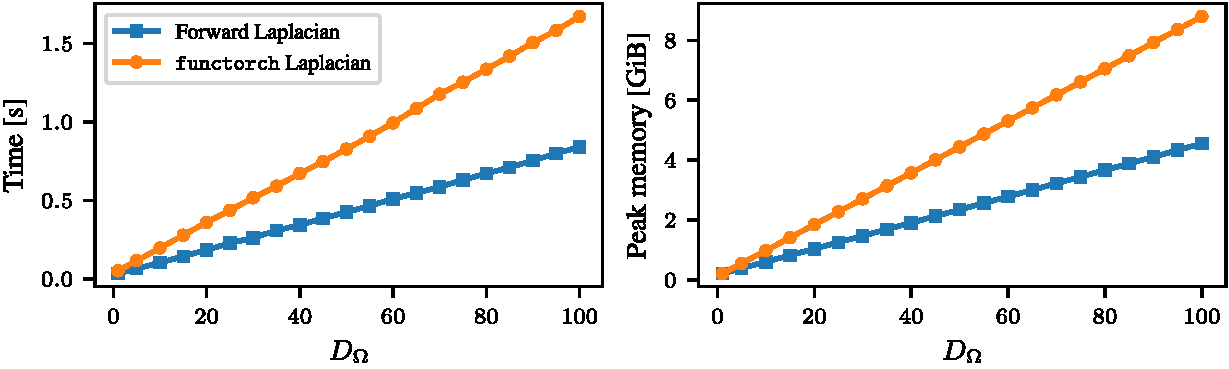
\includegraphics[width=\linewidth]{../figures/laplacian_benchmark.pdf}
  \caption{Time (left) and memory (right) required with the forward Laplacian used in our implementation and the \texttt{functorch} implementation; we find that for both methods both measures of complexity grow linearly in the input dimension.}
  \label{app:fig:comparison}
\end{figure}

\paragraph{Other scalings}
Both the forward Laplacian and nested backpropagation scale linearly w.r.t. batch size.
Scaling w.r.t. output dimension (as asked by TQnM) is less relevant as many high-dimensional PDE problems are scalar-valued.
Scaling w.r.t. number of trainable parameters is highly architecture-dependent. This is also true for simple backpropagation in standard deep learning applications and we believe this question needs to be answered on a case-by-case basis.


%%% Local Variables:
%%% mode: latex
%%% TeX-master: "../main"
%%% End:
